\section{Patientgruppe}
\textit{Følgende afsnit omhandler omfanget af knæartrose. Afsnittet redegør for patientgruppen samt de forskellige disponeringsfaktorer for lidelsen. Ydermere vil patienternes forløb blive beskrevet og den sidste fase vil blive analyseret. Dette vil danne grundlag for at klassificere gruppen af patienter, som tilbydes en TKA-operation.}
%\subsection{Demografi}
%En længere række faktorer har betydning for udviklingen af artrose. Hvis en eller flere af disse faktorer er tilstede, er den påvirkede mere disponeret for knæartrose. Dette er eksempelvis, overbelastning igennem arbejde og fritid, tidligere knæskader, genetisk arv, overvægt samt køn \citep{brostrom2012}. Knæartrose er til stede blandt 45\% af alle 80-årige i befolkningen. Antallet af personer med knæartose kan formodes at stige da levealderen i Danmark stiger. Dette er ikke det eneste faktor, hvorfor prævalensen kan antages at stige. En af risikofaktorerne for udviklingen af knæartrose er overvægt, hvilket 47\% af den danske befolkning kan kategoriseres som. Ydermere stiger andelen af overvægtige med alderen, hvilket ligeledes er tilfældet for knæartrose. Overvægtige med en høj body-mass-index (BMI>30\citep{definitionfedme1999}) er disponeret for knæartrose med en relativ risiko på en faktor tre, hvoraf en kombination af ovenstående faktorer øger risikoen for lidelsen. Dog kan der opstå problematikker vedrørende benyttelsen af BMI, da metoden ikke skelner mellem fedt og muskler. \citep{brostrom2012} \citep{Vestergaard2014} \citep{Vestergaard2016} \citep{Lind2016} \citep{Lind2016b}

\subsection{Behandlingsforløb}
Behandlingsforløbet for en patient med knæartrose består af flere metoder. Målet med behandling af knæartrose er smertelindring, mobilitetsforøgelse samt forebyggelse. Generelt kan metoderne inddeles i non-invasive og invasive. Metodevalget afhænger af sygdommens omfang.

\begin{figure}[H]
	\centering
	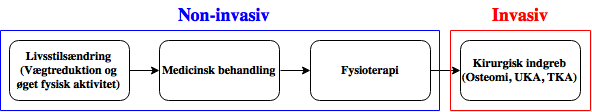
\includegraphics[width=1\textwidth]{figures/bProblemanalyse/flowchart_behandlingsforloeb.png}
	\caption{Flowchartet viser de forskellige behandlingsmetoder, en patient med knæartrose gennemgår. Livsstilsændring dækker eksempelvis vægtreduktion, men medicinsk behandling er smertelindrende stoffer og kirurgiske indgreb er eksempelvis alloplastikker.}
	\label{fig:flow_behandlingsfaser}
\end{figure}\vspace{-.25cm}

Som det ses på \figref{fig:flow_behandlingsfaser}, består første metode af en livsstilsændring, hvor en vægtreduktion samt øget fysisk aktivitet kan afhjælpe patientens symptomer. Hvis dette ikke er tilstrækkeligt, kan medicinsk behandling i form af smertelindrende medikamenter benyttes, enten som enkeltstående behandling eller sideløbende med fysioterapi, der har til formål at styrke muskulaturen omkring leddet. Hvis de non-invasive behandlingsmetoder ikke afhjælper lidelsen i en grad hvor patienten er tilfreds, kan invasive metoder anvendes. Ved en sådan overvejelse vurderes den diagnosticerede grad af artrose, ud fra den kliniske vurdering og radiologiske forandringer i knæet fundet ved røntgenbilleder. Baggrunden for at den kliniske vurdering skal verificeres forud for kirurgi er, at smerte fra hofte og ryg kan projiceres til knæet. Hermed tilbydes patienten først en TKA-operation, når non-invasive behandlingsmetoder ikke har lindret symptomer i en tilstrækkelig grad. \citep{Lind2016b} \citep{brostrom2012} \citep{skou2016}

%noter: 
%første section under billedet
%hvad er “overkommelige symptomer” ? Pia vill nok spørge…
%sidste sætning er udødvendig: vi har tidligere sagt at graden af artrose skal diagnosticeres så der vil det vel bedømmes om patienten har moderat til svær artrose. 

\subsection{Postoperative TKA resultater}
I 2014 blev der udført cirka 9.800 TKA-operationer, hvoraf 1,8\% af disse var revisioner et år efter primæroperationen. \citep{aarsrapport2016} Et studie af \citer{Petersen2015} viste, at der var 19\% af patienterne efter primær TKA havde svære til uudholdelige smerter. Det samme var gældende for 47\% af patienterne der fik en revision. \citer{Petersen2015} viste ligeledes, at 11\% af patienterne med primær- og 25\% af patienterne med revisionsoperationen ikke var tilfredse med operationen. \citep{Petersen2015} Herved antydes en skævhed i forholdet mellem patienter med smerter og utilfredse patienter. \\
I 2012 viste en undersøgelse fra Sundhedsstyrelsen, at 81 til 85\% af patienter, der havde modtaget en primær TKA-operation, var tilfredse, 8 til 11\% var decideret utilfredse og resten var i tvivl eller til dels utilfredse. Resultatet heraf er, at op mod 19\% af patienterne ikke opnår bedring fra deres smerter og eventuel nedsat mobilitet. \citep{brostrom2012} Sundhedsstyrelsens indikationer vedrørende patientutilfredshed understøttes af flere internationale studier. Eksempelvis fandt studiet af \citer{Bourne2010}, at 19\% af de undersøgte patienter var utilfredse med resultatet af deres TKA-operation. Ydermere viser undersøgelser på tværs af tilsvarende studier, at andelen af utilfredse patienter befandt sig i området 11 til 25\%. \citep{Bourne2010} Et studie af \citer{Jacobs2014} undersøgte, om der er nogle bestemte karakteristika for patienter, som er utilfredse efter deres TKA-operation. \citer{Jacobs2014} fandt, at hverken alder, køn eller BMI havde en signifikant sammenhæng med om patienten var tilfreds eller utilfreds. 
%\begin{table}[H]
%	\centering
%\begin{tabular}{ccc}
%	\hline
%	\rowcolor[HTML]{C0C0C0} 
%	Studie            & Forsøgspopulation {[}N{]} & Utilfreds {[}\%{]} \\ \hline
%	Anderson et al.   & 74                        & 11                 \\
%	Noble et al.      & 253                       & 25                 \\
%	Robertsson et al. & 27.372                    & 18                 \\
%	Wylde et al.      & 228                       & 15                 \\
%	Hawker et al.     & 1193                      & 15                 \\
%	Heck et al.       & 291                       & 12                 \\
%	Bourne et al.     & 1703                      & 19                 \\
%	Petersen et al.	  & 215						  & 11				   \\ \hline
%\end{tabular}
%	\caption{I tabellen ses \cite{Bourne2010} sammenligning af flere studiers resultater vedrørende patientutilfredshed efterfulgt en primær TKA-operation. \citep{Bourne2010}\citep{Petersen2015}}
%	\label{tab:patient_utilfreds}
%\end{table}

\citer{Sakellariou2016} har undersøgt, hvor stor en andel af patienterne, der oplever kroniske postoperative smerter efter en TKA-operation. Udfra resultaterne viste \citer{Sakellariou2016}, at op mod 39\% af studiets patienter oplevede moderat til alvorlig smerte, et år efter TKA-operationen. Der kan ikke drages en parallel mellem smerte og ovennævnte utilfredshed; kroniske postoperative smerter kan stadig være en lindring af patientens præoperative smerte. Patienter kan desuden være utilfredse af andre grunde end posoperative kroniske smerter, som eksempelvis funktionsnedsættelse \citep{Jacobs2014}. Dette kan ses af \citer{Skallariou2016}, hvor kun 19\% af patienterne var utilfredse, mens 39\% af patienterne oplevede smerter.\citep{Sakellariou2016} 

I et studie af \citer{Jacobs2014} var størstedelen den utilfredse forsøgspopulations utilfredshed relateret til enten passiv fleksion, smerte eller funktionsnedsættelse. De præoperative tests indikerede, at der ikke var signifikant forskel vedrørende smerte(p=0,53) eller funktion(p=0,62), blandt de to grupper af patienter som postoperative var tilfredse eller utilfredse. Postoperativt blev samme test udført, og her var der signifikant forskel (p=<0,001) ved alle indikationer; passiv fleksion, smerte og funktion. 
De patienter som postoperativt var i den utilfredse gruppe, havde signifikant dårligere resultater af operationen, i forhold til patienter i den tilfredse gruppe, hvormed dette kan antages som værende grunden til patienternes utilfredshed. \citep{Jacobs2014} 
Dette fund understøttes ligeledes af studiet af \cite{Bourne2010}, hvis resultater indikerer at de utilfredse patienter har signifikant flere smerter, led stivhed samt nedsat funktion et år efter operationen, sammenholdt med gruppen af tilfredse patienter. \citep{Bourne2010}

Patientgruppen som postoperativt er utilfredse er svært definerbar. Problematikken opstår i og med klassificeringen bag de potentielt 11 til 25~\% utilfredse patienter er vedrørende postoperative smerte samt funktion. Det kan forestilles at der blandt nogle af patienterne findes en forventningsfaktor, hvilket gør de postoperativt kategoriserer sig selv som værende utilfreds, omend de rent faktisk har opnået en forbedring af både smerte og eller mobilitet. Det kan tænkes at forventningsfaktoren kan være medvirkende til at patienterne ikke oplever den forbedring de havde stillet sig i vente, hvorved de ville kategorisere sig som værende utilfredse. Denne antagelse understøttes af \cite{Bourne2010}, som beskriver de største prædiktorer for utilfredshed efter en TKA-operation. Den største faktor er, at patientens forventninger til operationen ikke er mødt, hvilket medfører 10,7 gange større risiko for utilfredshed. \citep{Bourne2010} I et andet studie af \cite{Keudell2013} bliver patienternes alder sammenkoblet med deres forventninger. Det tyder på at den ældre patientgruppe (>65 år) har generelt har lavere forventninger til operationsresultatet, end den yngre patientgruppe (<55 år). I dette studie indikeres det at den ældre patientgruppe generelt har større tilfredshed, end den yngre.\cite{Bourne2010} Dette kan antages at have en sammenhæng med et øget aktivitets behov hos yngre patienter. 

%Dette kan antages at have en sammenhæng med påstanden fra \cite{Bourne2010}, vedrørende prædiktoren til utilfredshed, omhandlende forventninger til operationen. \textbf{NOTE:(7 (mangler analyse?))}

Knæartrose er en lidelse i vækst da den umiddelbare disponerede målgruppe er voksende. Resultatet heraf medfører at antallet af registrerede tilfælde med symptomer sandsynligvis ligeledes vil stige, og der i fremtiden vil blive udført flere operationer, hvoraf det kan antages at der vil forekomme flere patienter med kroniske smerter postoperativt TKA, uden mulighed for yderligere behandling.

